\documentclass[12pt,twoside]{article}

\usepackage{amsmath}
\usepackage{fancyhdr}
\usepackage{graphicx}
\usepackage{amssymb}
\usepackage[colorlinks=true, linkcolor=red, urlcolor=blue, citecolor=blue]{hyperref}



\setlength{\oddsidemargin}{0pt}
\setlength{\evensidemargin}{0pt}
\setlength{\textwidth}{6.5in}
\setlength{\topmargin}{0in}
\setlength{\textheight}{8.5in}
\setlength{\headheight}{15pt}

\newcommand{\andrew}{Andrew Xia}
\newcommand{\name}{6.115 Final Project Lab Notebook}
\renewcommand{\thesubsection}{\thesection.\alph{subsection}}
\renewcommand{\sectionmark}[1]{\markboth{#1}{}} % set the \leftmark


\pagestyle{fancy}
\fancyhead[R]{\andrew}
\fancyhead[L]{\leftmark} % 1. sectionname
\fancyhead[C]{\name}


\begin{document} 
\begin{center} {\bf \Large \name}
\\ \emph{Hardware Implementation of Tinder}
\\ {\bf \andrew}
\end{center}
\section{Overview}
For my final project, I hope to build a 3D touchless tracking interface and connect it with my 8051 and PSoC to allow users to play 3D tic tac toe with either each other or a computer AI. 
\\
\\ \emph{What interested you in the idea?} I am interested in this idea because I want to work on a project that has both an interesting and flashy hardware and software component. Writing the AI software for my 3D tic tac toe board will be a very rewarding and educational experience for me, and building the 3D tracing interface will also be very fun. 
\\ 
\\ \emph{Why is this project interesting?} This project is interesting because while 2D tic tac toe is a game familiar to all, 3D tic tac toe represents a game that while it is familiar, it can also be novel and entertaining. This project also uses a 3D touchless interface for user input, which is another novel way of interacting with software, as we are used to touching buttons or screens to communicate with devices in our daily lives. 

\subsection{Hardware Overview}
The key hardware component of my project will be building a 3D touchless interface, which is shown in the image to the side. The three aluminum foils (or a similar material) on the three sides are the capacitors that the human finger complements, and thie distance from each of the three capacitors will definite the capacitance of the capacitance, which we can measure using an ADC, and effectively pinpoint the 3D location of the human hand. 
\\ I will use a 74LS245 chip to connect my PSoC to a VGA cable which can then display information on a screen. I will use what was covered in lecture to complete this task. 
\\ Below is a preliminary hardware schematic of my final project:
\begin{center}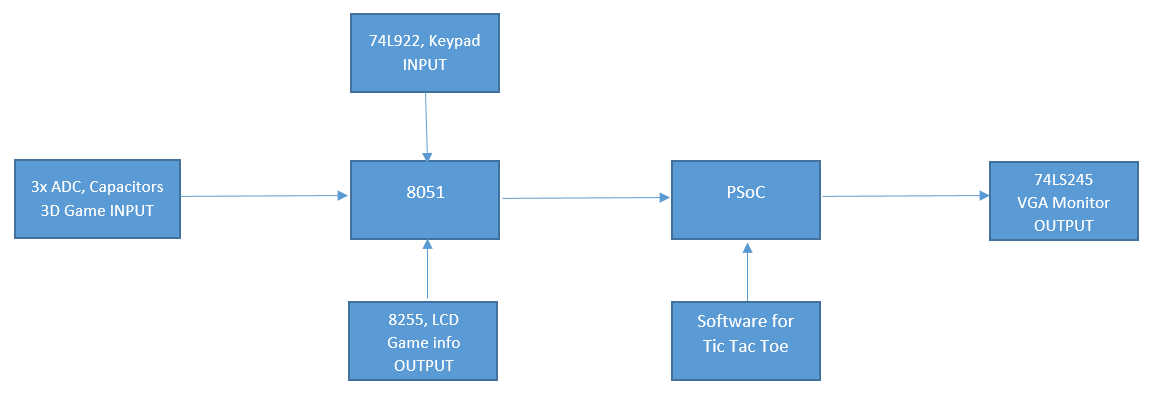
\includegraphics[width = 120mm]{../Proposals/Hardware_final.png} \end{center}

\subsection{Software Overview}
As for my software, I will code my project in C, using the PSoC as my main control module, as it would would be more efficient to do so over writing code in assembly for the 8051. The Tic Tac Toe AI is not too software heavy, so I hope to develop the basic framework for my code and spend the rest of my extra time focusing on hardware improvements. 
\\ Here is the high level software workflow for my final project:
\begin{center}\fbox{\begin{minipage}{35em}

\begin{enumerate}
\item Initiate \& Reset Tic Tac Toe Board
\item Mode 1: two player Tic Tac Toe
	\begin{enumerate}
	\item User can view \& rotate, using 74L922 or capacitive-based sensors, current 3D tic tac toe board on VGA display
	\item User adds piece to the board by leaving hand in position of 3D touchless tracking interface for extended amound of time
	\item After entering piece on board, the other player can play. 
	\end{enumerate}
\item Mode 2: one player AI Tic Tac Toe
	\begin{enumerate}
	\item User can view \& rotate, using 74L922 or capacitive-based sensors, current 3D tic tac toe board on VGA display
	\item User adds piece to the board by leaving hand in position of 3D touchless tracking interface for extended amound of time
	\item After entering piece on board, computer plays against user and submits his move through AI algorithm. 
	\end{enumerate}
\item Reset the game and enter either mode through the 74C922 Keypad
\end{enumerate}

\end{minipage}} \end{center}

\subsection{Format of my Lab Notebook}
I plan on formatting my lab notebook in this latex file, in which each day I work on the lab will be a section, and I can also reorganize my lab notebook to be thematically organized by the module that I will work on. 
\\ Each day, or section, will contain an {\em introduction} section in which I discuss the goals that I have for the day, and I will detail the tasks that I will work on in the subsections for each day. 

\newpage
\section{April 21, 2016}
Goals I have for today / {\bf done} if task completed
\begin{itemize}
\item Set up github for version control of my lab notebook and code {\bf done}
\item Build my initial capacitance based sensor
\item Set up my computer so I can code in C
\end{itemize}

\subsection{Setting up github}
I am following the tutorial \href{https://help.github.com/articles/adding-an-existing-project-to-github-using-the-command-line/}{here} to create a new github repository. It will be located in my 6.115 dropbox folder, and on my github account under the repository \href{https://github.com/qandrew/6.115-final-project}{6.115-final-project}

\subsection{Building my initial capacitance based sensor}
References include this \href{http://makezine.com/projects/a-touchless-3d-tracking-interface/}{Makezine link}. 
\\ Notes on building a capacitance based sensor:
\begin{enumerate}%[itemsep=5mm]
\item Beacuse humans have very little capacitance $~ 10 pF$, the time constant to which the plate would charge up based on the distance of the finger to the plate should be very small. Thus, I may need to think of more intelligent methods to build an effective capacitance based sensor. 
\item I can design different circuits
\end{enumerate}

\subsection{Setting up my computer}
To install {\bf C}, I am following this \href{https://en.wikibooks.org/wiki/C_Programming/What_you_need_before_you_can_learn}{website} to install a C compiler for my computer. 
\\
\\ To install the Cypress PSoC creator IDE, I am following the instructions \href{http://www.cypress.com/products/psoc-software}{here}. Having PSoC Creator on my computer should help increase my productivity and workflow. 

\end{document}